\documentclass[a4paper,12pt]{report}
\usepackage[utf8]{inputenc}
\usepackage{enumitem} %permite el uso de letras para enumerar
\usepackage{graphicx} %para las imagenes
\usepackage{float} %para fijar las imagenes
\usepackage{amsmath} %para centrar ecuaciones

\usepackage{tikz}
\usetikzlibrary{arrows.meta, positioning} %para hacer diagramas de bloques

\usepackage{amsmath}%para entornos de alineacion
\usepackage{amsfonts}%para las letras lindas de matematica
\setlength{\jot}{8pt}%modifica el interlineado

\usepackage{tikz} %Libreria para graficos
\usetikzlibrary{calc, arrows.meta, positioning}

\usepackage[a4paper, %margenes de pagina
  left=2.5cm,
  right=2.5cm,
  top=2cm,
  bottom=2cm,
  includehead
]{geometry}

\usepackage{fancyhdr}
\pagestyle{fancy}
\lhead{UTN-FRC}
\chead{ASyS}
\rhead{2R3}
\cfoot{\thepage}
\setlength{\headwidth}{\textwidth} % Hace que el ancho del encabezado coincida con el ancho del texto
\setlength{\headheight}{15pt}  % Ajusta la altura del encabezado
\setlength{\headsep}{20pt}     % Ajusta la separación entre el encabezado y el contenido

\usepackage{titlesec}
\titleformat{\chapter}[display]
  {\normalfont\Large\bfseries}{}{0pt}{}
\titlespacing*{\chapter}{10pt}{-45pt}{10pt}

\usepackage{etoolbox} 
\makeatletter
\patchcmd{\chapter}{\thispagestyle{plain}}{\thispagestyle{fancy}}{}{} %Muestra encabezado en las paginas con \chapter
\makeatother

%Comandos de fake section y fake sub section, para poder agregar secciones al indice
\newcommand{\fs}[1]{%
  \par\refstepcounter{section}% Increase section counter
  \sectionmark{#1}% Add section mark (header)
  \addcontentsline{toc}{section}{\protect\numberline{\thechapter.\alph{section}}#1}% Add section to ToC
}
\newcommand{\fss}[1]{%
  \par\refstepcounter{subsection}% Increase subsection counter
  \subsectionmark{#1}% Add subsection mark (header)
  \addcontentsline{toc}{subsection}{\protect\numberline{\alph{subsection}}#1}% Add subsection to ToC
}

\renewcommand{\contentsname}{Tabla de Contenidos}

\title{%
\setlength{\headwidth}{\textwidth} % Hace que el encabezado tenga el mismo ancho que el contenido
\setlength{\headheight}{15pt}  % Ajusta la altura del encabezado
\setlength{\headsep}{10pt}     % Ajusta la separación entre el encabezado y el contenido
  \fontsize{25}{0}\selectfont Universidad Tecnológica Nacional \\
  \fontsize{22}{30}\selectfont Analisis de Señales y Sistemas \\
  \fontsize{20}{25}\selectfont Trabajo Practico 3
}
\author{
Franco Palombo\\
Ignacio Gil\\
Laureano Valentin Reinoso\\
Luciano Tomas Cortesini Perez\\
}
\date{19 / 08 / 2024}

\begin{document}

\maketitle
\tableofcontents
\thispagestyle{plain}

\chapter{Ejercicio 1}
Graficar ambas señales superpuestas, y verificar cuántas muestras de tiempo discreto se corresponden con el rango de
tiempo continuo utilizado para la representación gráfica.

\begin{enumerate}[label=\alph*), left=0pt]

  \item \fs{} Una señal analógica $x(t) = e^{-2t} \mu(t)$ se muestrea para generar la secuencia de tiempo discreto 
    $x[n]$, considerar $n = nT_s$, con $T_s = 0.05$, $T_s = 0.01$, $T_s = 0.1$.

    \begin{figure}[H]
      \centering
      \begin{minipage}{0.55\textwidth}
        \centering
        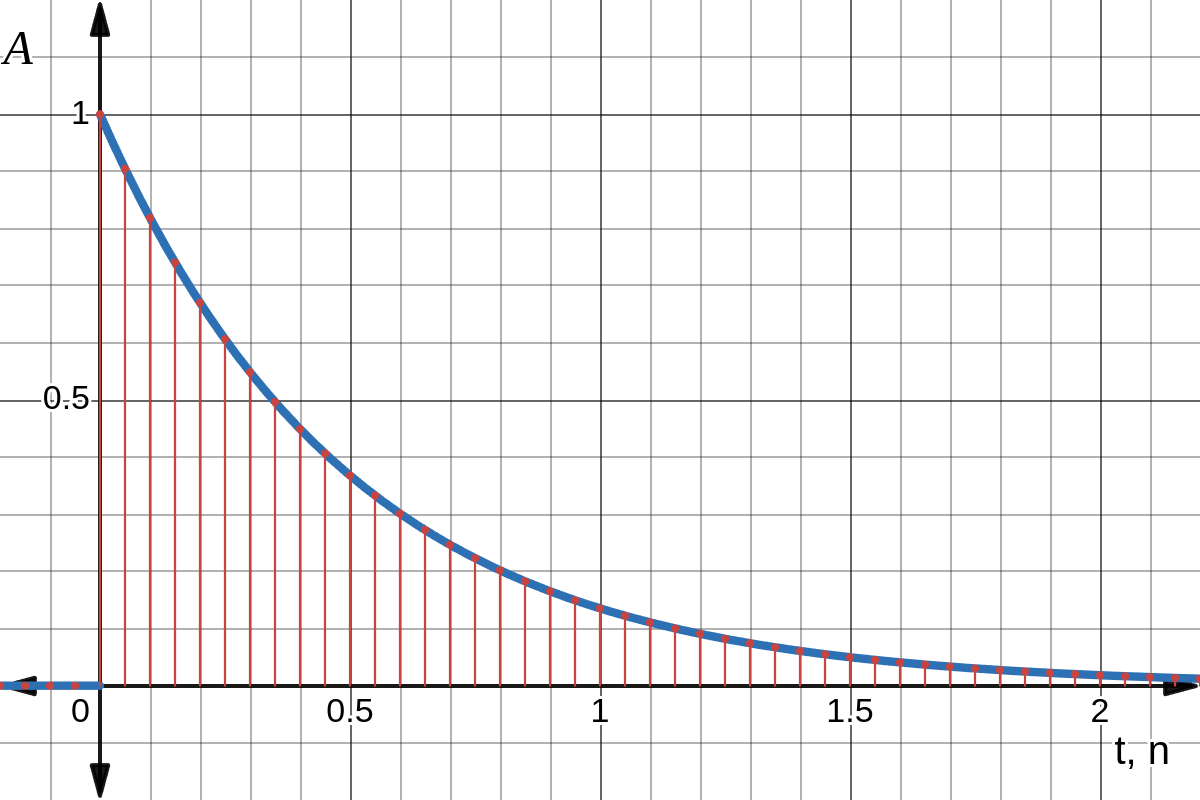
\includegraphics[width=1\textwidth]{./images/ej1.1.png}
        \textit{Muestreo con $T_s=0.05$\\Muestas en el intervalo: $48$}
      \end{minipage}
    \end{figure}

    \begin{figure}[H]
      \centering
      \begin{minipage}{0.55\textwidth}
        \centering
        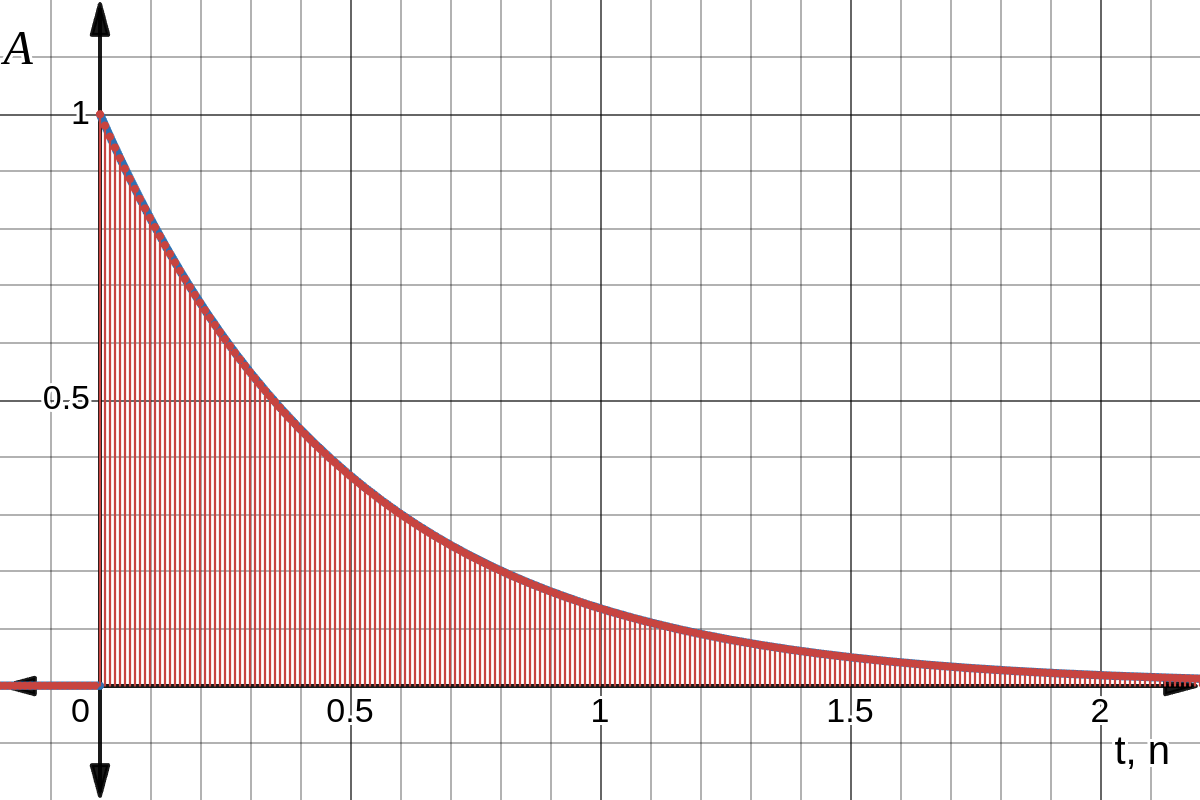
\includegraphics[width=1\textwidth]{./images/ej1.2.png}
        \textit{Muestreo con $T_s=0.01$\\Muestas en el intervalo: $140$}
      \end{minipage}
    \end{figure}

    \begin{figure}[H]
      \centering
      \begin{minipage}{0.55\textwidth}
        \centering
        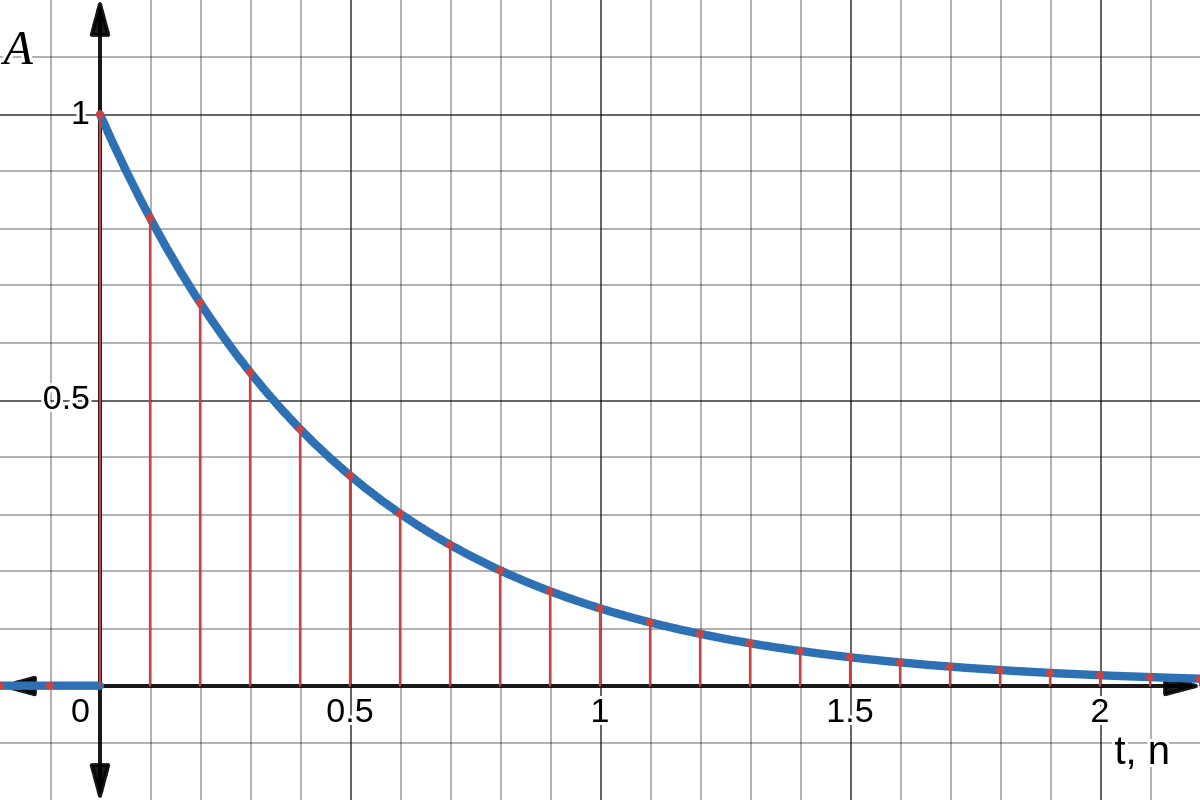
\includegraphics[width=1\textwidth]{./images/ej1.3.png}
        \textit{Muestreo con $T_s=0.1$\\Muestas en el intervalo: $24$}
      \end{minipage}
    \end{figure}


  \item \fs{} Una señal analógica $x(t) = 10 \cos(2t) \mu(t)$ se muestrea para generar la secuencia de tiempo discreto
    $x[n]$, con $T_s = 0.1$ y $T_s = 0.01$.

    \begin{figure}[H]
      \centering
      \begin{minipage}{0.55\textwidth}
        \centering
        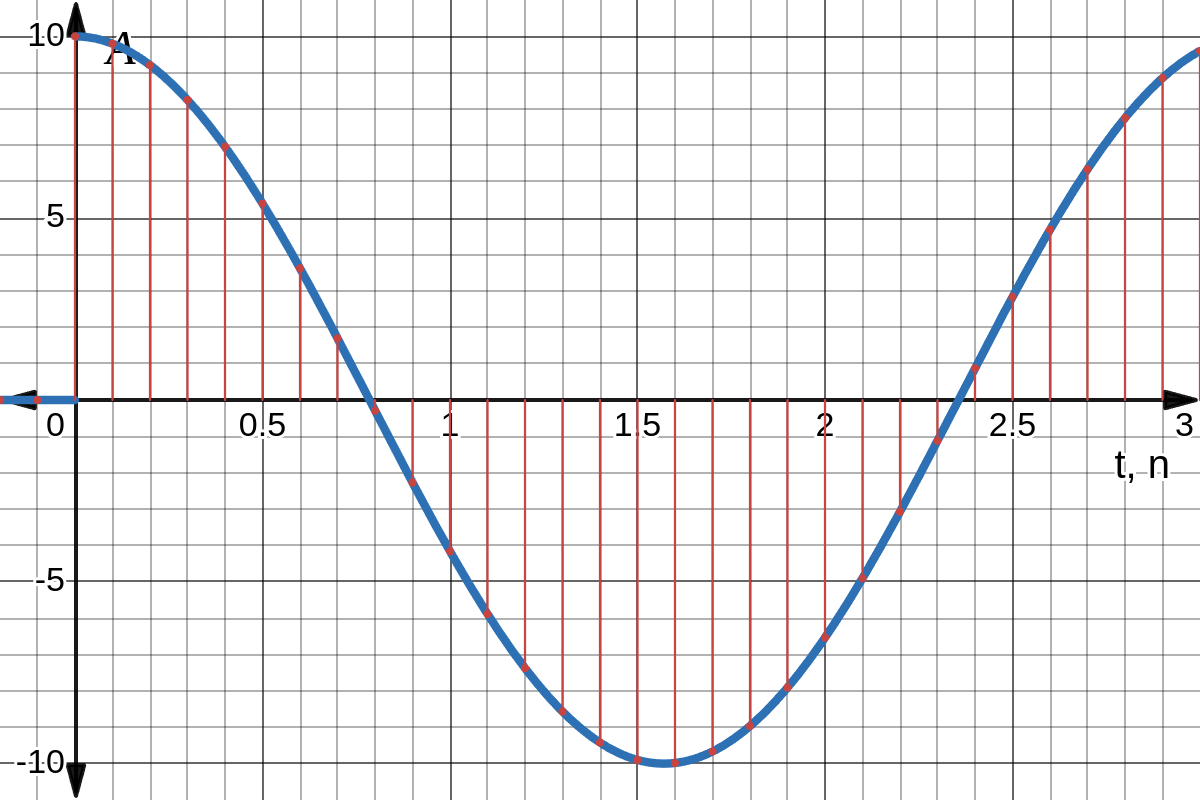
\includegraphics[width=1\textwidth]{./images/ej1.4.png}
        \textit{Muestreo con $T_s=0.1$\\Muestas en el intervalo: $32$}
      \end{minipage}
    \end{figure}

    \begin{figure}[H]
      \centering
      \begin{minipage}{0.55\textwidth}
        \centering
        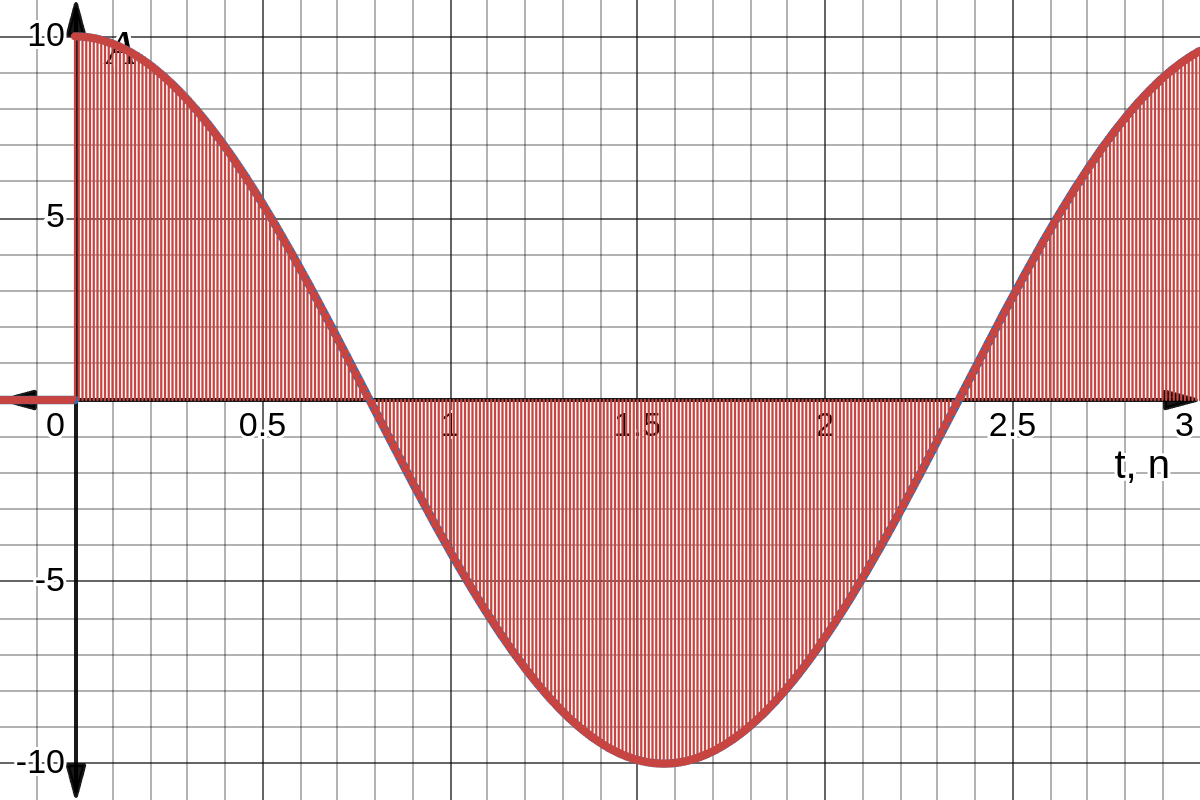
\includegraphics[width=1\textwidth]{./images/ej1.5.png}
        \textit{Muestreo con $T_s=0.01$\\Muestas en el intervalo: $320$}
      \end{minipage}
    \end{figure}

  \item \fs{} Considerar a continuación una secuencia de valores obtenida de una adquisición de datos en un proceso de
    muestreo. Describir una expresión matemática que permita involucrar la secuencia temporal del proceso de adquisición.
    Considerar la secuencia causal:

    \[
    \{0, 3.4, 6, 7, 8.5, 10, 13.4\}
    \]

    Para encontrar una funcion que pase por todos los puntos de la secuencia, como una forma de aproximar la señal en el
    dominio temporal de la cual se obtuvo la secuencia, utilizamos el metodo de interpolación de Lagrange. Definido por:

    $$f(t)= \sum_{j=0}^n f[j] \prod_{i=0,i \neq j}^{n} \frac{t - t_i}{t_k - t_i}$$
    Donde:

    \centering
    \begin{minipage}{0.5\textwidth}
      $n$: número de elementos de la secuencia\\
      $f[k]$: el elemento k-esimo de la secuencia\\
      $t_i$: el instante temporal del elemento i-esimo
    \end{minipage}

    \begin{figure}[H]
      \centering
      \begin{minipage}{0.55\textwidth}
        \centering
        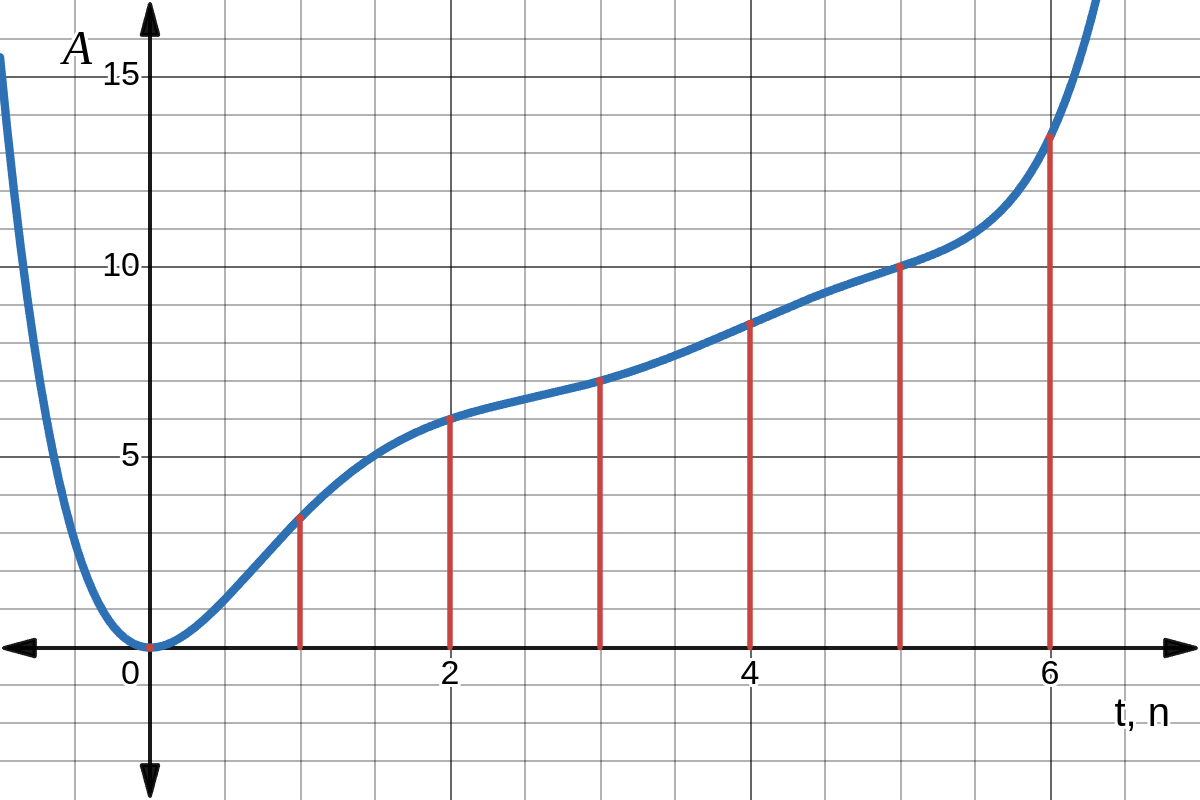
\includegraphics[width=1\textwidth]{./images/ej1.6.png}
        \textit{Interpolación por polinomio de Lagrange}
      \end{minipage}
    \end{figure}

\end{enumerate}

\chapter{Ejercicio 2}
Considerar el siguiente sistema de tiempo discreto:

\begin{figure}[h]
  \centering
  \begin{tikzpicture}[auto, node distance=2cm, >=Stealth, thick]
    % Definición de estilos para los bloques y el sumador
    \tikzstyle{block} = [draw, rectangle, minimum height=1.5em, minimum width=3em]
    \tikzstyle{sum} = [draw, circle, inner sep=1pt, minimum size=0.7cm, node distance=2cm]
    \tikzstyle{connector} = [fill, circle, minimum size=4pt, inner sep=0pt] % Estilo para el punto de conexión

    % Definición de nodos
    \node at (0,-3) [coordinate] (input) {}; % Nodo de entrada x(n)
    \node [connector, right=2cm of input] (c1) {};
    \node [block, right=1cm of c1, yshift=1.5cm] (h1) {$h_1[n]$};
    \node [block, right=1cm of h1] (h2) {$h_2[n]$};
    \node [sum, right=0.5cm of h2, yshift=-1.45cm] (sumador) {$\Sigma$}; % Nodo del sumador
    \node [block, right=1cm of sumador] (h3) {$h_3[n]$}; % Bloque h3
    \node [coordinate, right=2cm of h3] (output) {}; % Nodo de salida y(n)
    \node [block, below=1cm of c1, xshift=2.8cm] (h4) {$h_4[n]$}; % Nodo de h4, en paralelo

    \draw[->] (input) -- node{$x[n]$}(c1);
    \draw[->] (c1) |- (h1);
    \draw[->] (h1) -- (h2);
    \draw[->] (h2) -| node [left, pos=0.9] {$+$} (sumador);
    \draw[->] (sumador) -- (h3);
    \draw[->] (h3) -- node {$y[n]$} (output);
    \draw[->] (c1) |- (h4); % Conexi+n del input hacia h4
    \draw[->] (h4) -| node[pos=0.9] {$-$} (sumador); % Conexión desde h4 hacia el sumador con signo negativo

  \end{tikzpicture}
\end{figure}

\begin{enumerate}[label=\alph*), left=0pt]

  \item\fs{} Si $h_1[n] = h_2[n] = 3^{-n}\mu[n]$, $h_3[n] = \mu[n]$, $h_4[n] = 2^{-n}\mu[n]$:

    La respuesta al impulso del sistema corresponde a:
    \begin{align*}
      h[n]&=(h_1[n]*h_2[n] - h_4[n])*h_3[n]\\
      h[n]&=(3^{-n}\mu[n]*3^{-n}\mu[n] - 2^{-n}\mu[n])*\mu[n]\\
      h[n]&=(3^{-n}(n-1)\mu[n] - 2^{-n}\mu[n])*\mu[n] \\
      h[n]&=3^{-n}n\mu[n]*\mu[n] - 3^{-n}\mu[n]*\mu[n] - 2^{-n}\mu[n]*\mu[n]\\
      h[n]&=\sum_{k=0}^n 3^{-k}k - \sum_{k=0}^n 3^{-k} - \sum_{k=0}^n 2^{-k}
    \end{align*}

    La serie geometrica:
    \begin{equation}
      \label{s.geometrica}
      \sum_{k=0}^{n} r^k = \frac{1-r^{n+1}}{1-r}
    \end{equation}
    Va a ayudarnos a resolver la segunda y tercera sumatoria. Sin embargo, para la primera vamos a necesitar
    manipularla.\\
    Primero derivamos la expresión anterior respecto a r.
    $$\sum_{k=0}^{n} kr^{k-1} = \frac{1-(n+1)r^{n} + nr^{n+1}}{(1-r)^2}$$
    Y finalmente multiplicamos por r.
    \begin{equation}
      \label{s.geometrica.deriv}
      \sum_{k=0}^{n} kr^k = \frac{r-(n+1)r^{n+1} + nr^{n+2}}{(1-r)^2}
    \end{equation}
    Con estos resultados, podemos continuar el desarrollo.

    {
      \allowdisplaybreaks
      \begin{align*}
        h[n] &= \left(\frac{\frac{1}{3}-(n+1)\left(\frac{1}{3}\right)^{n+1} + n\left(\frac{1}{3}\right)^{n+2}}{\left(1-\frac{1}{3}\right)^2} -
          \frac{1-\left(\frac{1}{3}\right)^{n+1}}{1-\frac{1}{3}} - \frac{1-\left(\frac{1}{2}\right)^{n+1}}{1-\frac{1}{2}}\right) \mu[n]\\
        %
        h[n] &= \left(-\frac{11}{4}-\frac{9}{4}(n+1)\left(\frac{1}{3}\right)^{n+1} + \frac{9}{4}n\left(\frac{1}{3}\right)^{n+2} -
        \frac{3}{2} \left(\frac{1}{3} \right)^{n+1} - 2 \left(\frac{1}{2}\right)^{n+1}\right) \mu[n] \\
        %
        h[n] &= \left(-\frac{11}{4} -\frac{3}{4} n 3^{-n} - \frac{3}{4} 3^{-n} +
          \frac{1}{4}n 3^{-n} - \frac{1}{2} 3^{-n} - 2^{-n}\right) \mu[n]\\
        %
        h[n] &= \left(-\frac{11}{4} - 2^{-n} - \frac{2}{4} n 3^{-n} - \frac{5}{4} 3^{-n}\right) \mu[n]
      \end{align*}
    }

    La respuesta al escalon unitario esta definida por:
    \begin{align*}
      y[n] &= \mu[n] * h[n]\\[6pt]
      %
      y[n] &= \sum_{k \in \mathbb{Z}} \left(-\frac{11}{4} - 2^{-n} - \frac{2}{4} n 3^{-n} - \frac{5}{4} 3^{-n}\right) \mu[k] \mu[n-k]\\
      %
      y[n] &= \mu[n] \sum_{k=0}^n \left(-\frac{11}{4} - 2^{-n} - \frac{2}{4} n 3^{-n} - \frac{5}{4} 3^{-n}\right)
    \end{align*}

    % desarrollo pambi
    %\begin{align*}
    %  y[n] &= \mu[n] * h[n]\\[6pt]
    %  y[n] &= \sum_{k \in \mathbb{Z}} \left(-\frac{11}{4} - \frac{5k}{4 \cdot 3^k} + \frac{9k}{4 \cdot 3^{(k+1)}} -
    %    \frac{9}{4 \cdot 3^{(k+1)}} + \frac{3}{2 \cdot 3^{(k+1)}} + \frac{2}{2^{(k+1)}} \right) \cdot \mu[k] \cdot \mu[n-k]\\[6pt]
    %  y[n] &= \mu[n] \cdot \sum_{k=0}^{n} \left(-\frac{11}{4} - \frac{5k}{4 \cdot 3^k} + \frac{9k}{4 \cdot 3 \cdot 3^k} -
    %    \frac{9}{4 \cdot 3 \cdot 3^k} + \frac{3}{2 \cdot 3 \cdot 3^k} + \frac{2}{2 \cdot 2^k} \right)\\[6pt]
    %  y[n] &= \mu[n] \cdot \sum_{k=0}^{n} \left(-\frac{11}{4} - \frac{5k}{4 \cdot 3^k} + \frac{3k}{4 \cdot 3^k} -
    %    \frac{3}{4 \cdot 3^k} + \frac{1}{2 \cdot 3^k} + \frac{1}{2^k}\right)
    %\end{align*}

    El desarrollo, ademas de largo, es engorroso y carece de la aplicacion de alguna propiedad importante o identidad
    no vista. Todos los terminos de la suma usan o la identidad de la serie trigonometrica (\ref{s.geometrica}), su
    derivada (\ref{s.geometrica.deriv}), o la identidad de una sumatoria constante. Como resultado, se obtiene lo
    siguiente:
    \begin{equation*}
      y[n] = \frac{5}{4} - \frac{11}{4} (n+1) + \frac{5n + 1}{8 \cdot 3^n} + \frac{3 (n+1)}{8 \cdot 3^n} -
        \frac{1}{2^n}
    \end{equation*}

    \begin{figure}[H]
      \centering
      \begin{minipage}{0.55\textwidth}
        \centering
        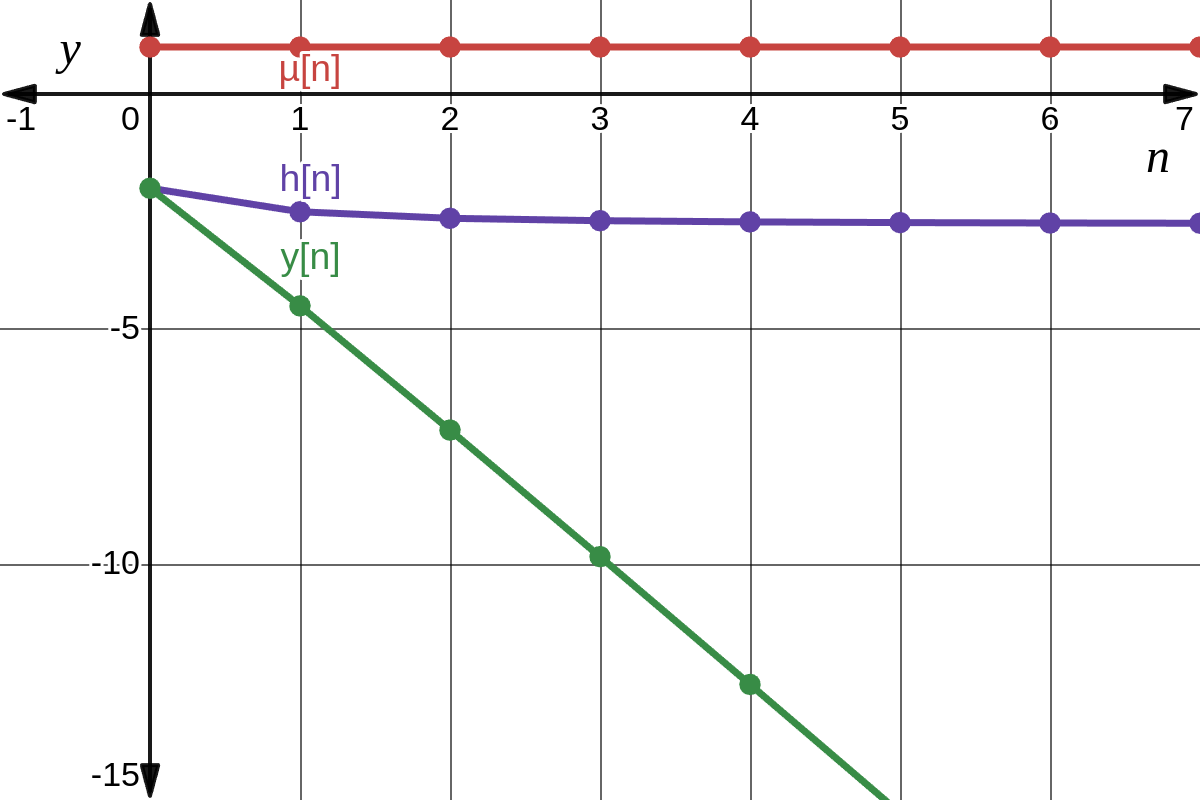
\includegraphics[width=1\textwidth]{./images/ej2.1.png}
        \textit{Grafica con las tres funciones discretas.}
      \end{minipage}
    \end{figure}

  \item \fs{} Si $h_1[n] = 2^{-n} u[n]$, $h_2[n] = \delta[n]$, $h_3[n] = h_4[n] = 3^{-n} u[n]$:

    La respuesta al impulso del sistema corresponde a:
    {
      \allowdisplaybreaks
      \begin{align*}
        h[n] &= (h_1[n] * h_2[n] - h_4[n]) * h_3[n]\\[6pt]
        h[n] &= (2^{-n} \mu[n] * \delta[n] - 3^{-n} \mu[n]) * 3^{-n} \mu[n]\\[6pt]
        h[n] &= (2^{-n} \mu[n] * 3^{-n} \mu[n] - 3^{-n} \mu[n] * 3^{-n} \mu[n])\\[6pt]
        h[n] &= \sum_{k \in \mathbb{Z}} \left(2^{-k} \cdot 3^{-(n-k)} \right) \cdot \mu[k] \cdot \mu[n-k] - \sum_{k \in \mathbb{Z}} \left( 3^{-k}
          \cdot 3^{-(n-k)} \right) \cdot \mu[k] \cdot \mu[n-k]\\
        h[n] &= 3^{-n} \cdot \mu[n] \sum_{k = 0}^n \left(2^{-k} \cdot 3^k\right) - 3^{-n} \cdot \mu[n] \sum_{k=0}^n \left(3^{-k} \cdot 3^{k}\right)\\[6pt]
        h[n] &= 3^{-n} \cdot \mu[n] \sum_{k = 0}^n \left(\frac{3}{2}\right)^{k} - 3^{-n} \cdot \mu[n] \sum_{k=0}^n 1
      \end{align*}
    }

    Aplicando la serie trigonometrica (\ref{s.geometrica}) y la serie de una constante, se obtiene el siguiente
    resultado:

    \begin{align*}
      h[n] &= -3^{-n} \left(2\left(1 - \left(\frac{3}{2}\right)^{n+1} \right) + (n+1)\right) \mu[n]\\[6pt]
      h[n] &= \left(-2 \cdot 3^{-n} + 2 \cdot 3^{-n} \cdot \left(\frac{3}{2}\right)^{n+1} -
        n \cdot 3^{-n} - 3^{-n}\right)\mu[n]
    \end{align*}

    La respuesta al escalón unitario esta definida por:
    \begin{align*}
      y[n] &= \mu[n] * h[n]\\[6pt]
      y[n] &= \sum_{k \in \mathbb{Z}} \left(-2 \cdot 3^{-k} + 2 \cdot 3^{-k} \cdot \left(\frac{3}{2}\right)^{k+1} -
        k \cdot 3^{-k} - 3^{-k}\right)\mu[k] \cdot \mu[n-k]\\[6pt]
      y[n] &= \mu[n] \sum_{k=0}^n \left(-2 \cdot 3^{-k} + 2 \cdot 3^{-k} \cdot \left(\frac{3}{2}\right)^{k+1} -
        k \cdot 3^{-k} - 3^{-k}\right)
    \end{align*}

    Nuevamente, aplicando las identidades de la serie geometrica (\ref{s.geometrica}), su derivada (\ref{s.geometrica.deriv})
    y la serie de una constante, se obtiene que:
    \begin{equation*}
      y[n] = \left(-9 \frac{1-\left(\frac{1}{3}\right)^{n+1}}{2} + 6 \left(1 - \left(\frac{1}{2}\right)^{n+1}\right) -
        \left(\frac{\frac{1}{3} - n\left(\frac{1}{3}\right)^{n} + (n-1) \left(\frac{1}{3}\right)^{n+1}}{\left(1-\frac{1}{3}\right)^{2}}+3^{-n}\cdot n\right)\right)
    \end{equation*}

    \begin{figure}[H]
      \centering
      \begin{minipage}{0.55\textwidth}
        \centering
        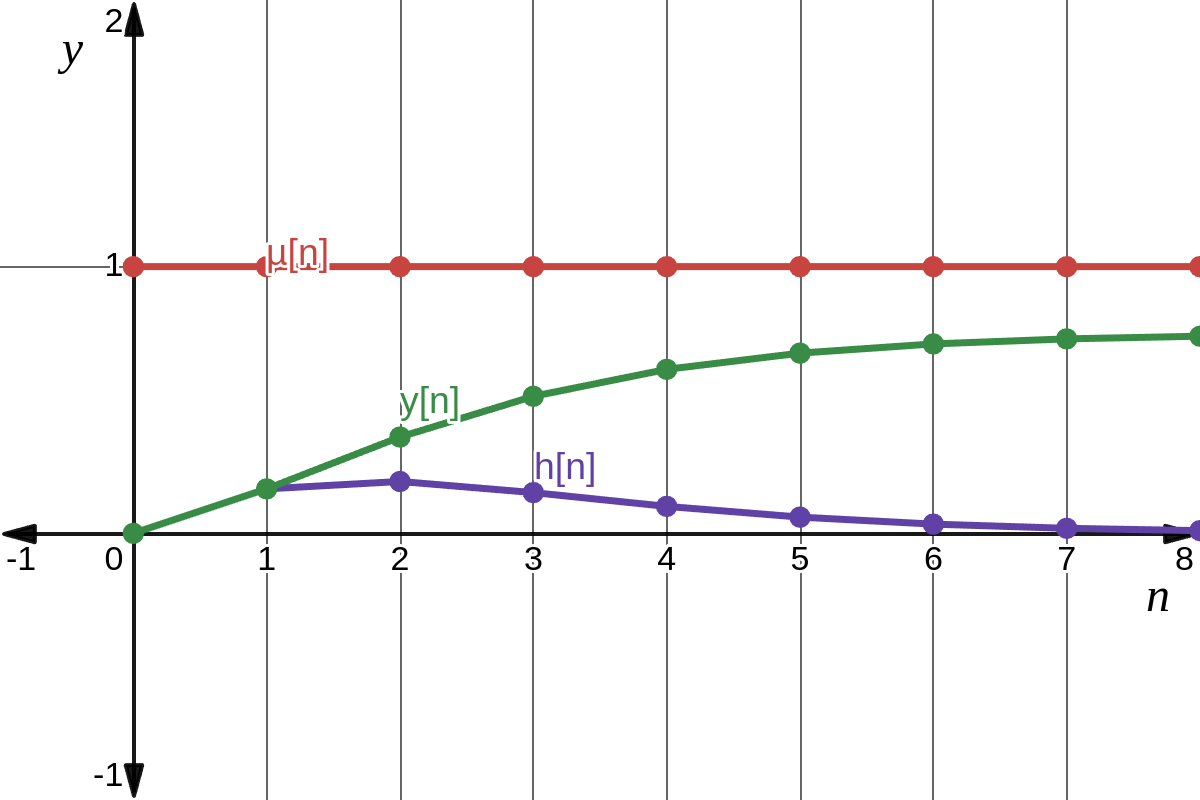
\includegraphics[width=1\textwidth]{./images/ej2.2.png}
        \textit{Grafica con las tres funciones discretas.}
      \end{minipage}
    \end{figure}

\end{enumerate}

\chapter{Ejercicio 3}
Considerar un sistema bancario de ahorro a tasa de interés mensual constante. Plantear el sistema considerando un 
depósito mensual constante en el mes $n$ de \$10, $r$ es la tasa de interés en el mismo periodo, y se considera el saldo
inmediatamente después del depósito en el periodo.

\begin{enumerate}[label=\alph*), left=0pt]
  \item \fs{} Identificar en el problema las variables de entrada y salida del mismo.
    % graficar sistema

  \item \fs{} Plantear un modelo en ecuaciones de diferencias capaz de caracterizar el sistema propuesto.

  \item \fs{} Representar la ecuación en diferencias por medio de un diagrama de bloques con retardos unitarios.

  \item \fs{} Evaluar el saldo para un periodo de capitalización de 48 meses.
\end{enumerate}

\chapter{Ejercicio 4}

\begin{enumerate}[label=\alph*), left=0pt]
  \item \fs{} Diagramar en un diagrama de bloques normalizado representativo del sistema para la siguiente ecuación en
    diferencias:

    \begin{align*}
      y_{[n+1]} + \frac{1}{2} y_{[n-1]} &= x_{[n]} + \frac{1}{2} x_{[n-1]}\\
      y_{[n+1]} &= x_{[n]} + \frac{1}{2} x_{[n-1]} - \frac{1}{2} y_{[n-1]}\\
      y_{[n]} &= x_{[n-1]} + \frac{1}{2} x_{[n-2]} - \frac{1}{2} y_{[n-2]}\\
      y_{[n]} &= D\{x_{[n]}\} + D^2\{\frac{1}{2} x_{[n]} - \frac{1}{2} y_{[n]}\}\\
    \end{align*}

    \begin{center}
      \begin{tikzpicture}[auto, node distance=2cm, >=Stealth, thick]
        % Definición de estilos para los bloques y sumador
        \tikzstyle{block} = [draw, rectangle, minimum height=1.5em, minimum width=3em]
        \tikzstyle{sum} = [draw, circle, inner sep=1pt, minimum size=1cm, node distance=2cm]
        \tikzstyle{connector} = [draw, fill, circle, minimum size=4pt, inner sep=0pt] % Estilo para el punto de conexión

        % Nodes
        \node at (0,0) [coordinate] (input){};
        \node [coordinate, on grid, right=3cm of input] (elbowInput1){};
        \node [block, on grid, below=1cm of elbowInput1] (signal1) {$\frac{1}{2}$};
        \node [connector, on grid, above=1.4cm of signal1](punto2){};
        \node [sum, on grid, below=2cm of signal1] (sum1) {$\sum$};
        \node [block, on grid, below=2cm of sum1] (signal2) {$- \frac{1}{2}$};
        \node [block, on grid, right=2cm  of sum1] (diferenciador1){$D$};
        \node [coordinate, on grid, right=7cm of input] (elbowInput2){};
        \node [block, on grid, below=1cm of elbowInput2] (signal3) {$1$};
        \node [sum, on grid, right=2cm of diferenciador1](sum2){$\sum$};
        \node [block, on grid, right=2cm of sum2](diferenciador2){$D$};
        \node [coordinate, on grid, right=4cm of diferenciador2](output){};
        \node [connector, on grid, right=1cm of diferenciador2](punto1){};
        \node [coordinate, on grid, below=2cm of punto1](elbowOutput1){};

        % Lines
        \draw [-] (input) -- node{$x_n(n)$} (elbowInput1);
        \draw [->] (elbowInput1) -- (signal1);
        \draw [-] (punto1) -- (elbowOutput1);
        \draw [->] (elbowOutput1) -- (signal2);
        \draw [-] (elbowInput1) -- (elbowInput2);
        \draw [->] (signal1) -- (sum1);
        \draw [->] (signal2) -- (sum1);
        \draw [->] (sum1) -- (diferenciador1);
        \draw [->] (diferenciador1) -- (sum2);
        \draw [->] (elbowInput2) -- (signal3);
        \draw [->] (signal3) -- (sum2);
        \draw [->] (sum2) -- (diferenciador2);
        \draw [->] (diferenciador2) -- node {$y_n(n)$}(output);

      \end{tikzpicture}
    \end{center}


  \item \fs{} Dado el sistema simulado por el diagrama de bloques a continuación, determinar la ecuación en diferencias
    que lo describe.

    \begin{center}
      \begin{tikzpicture}[auto, node distance=2cm, >=Stealth, thick]
        % Definición de estilos para los bloques y sumador
        \tikzstyle{block} = [draw, rectangle, minimum height=1.5em, minimum width=3em]
        \tikzstyle{sum} = [draw, circle, inner sep=1pt, minimum size=1cm, node distance=2cm]
        \tikzstyle{connector} = [draw, fill, circle, minimum size=4pt, inner sep=0pt] % Estilo para el punto de conexión

        % Nodes
        \node at (0,0) [coordinate] (input){};
        \node [coordinate, on grid, right=3cm of input] (elbowInput1){};
        \node [block, on grid, below=1cm of elbowInput1] (signal1) {$\frac{1}{2}$};
        \node [sum, on grid, below=2cm of signal1] (sum1) {$\sum$};
        \node [block, on grid, below=2cm of sum1] (signal2) {$-3$};
        \node [coordinate, on grid, below=1cm of signal2](elbowOutput3){};
        \node [block, on grid, right=2cm  of sum1] (diferenciador1){$D$};
        \node [coordinate, on grid, right=11cm of input] (elbowInput2){};
        \node [block, on grid, below=1cm of elbowInput2] (signal3) {$-5$};
        \node [sum, on grid, right=2cm of diferenciador1](sum2){$\sum$};
        \node [block, on grid, below=2cm of sum2] (signal4) {$3$};
        \node [coordinate, on grid, below=1cm of signal4](elbowOutput2){};
        \node [block, on grid, right=2cm of sum2](diferenciador2){$D$};
        \node [sum, on grid, right=2cm of diferenciador2](sum3){$\sum$};
        \node [coordinate, on grid, right=3cm of sum3](output){};
        \node [connector, on grid, right=1cm of sum3](punto1){};
        \node [coordinate, on grid, below=3cm of punto1](elbowOutput1){};
        \node [connector, on grid, below=3cm of sum2](nodo1){};
        \node [connector, on grid, above=3.4cm of sum1](nodo1){};

        % Lines
        \draw [-] (input) -- node{$x_n(n)$} (elbowInput1);
        \draw [->] (elbowInput1) -- (signal1);
        \draw [-] (punto1) -- (elbowOutput1);
        \draw [-] (elbowOutput1) -- (elbowOutput2);
        \draw [-] (elbowOutput1) -- (elbowOutput3);
        \draw [->] (elbowOutput3) -- (signal2);
        \draw [->] (elbowOutput2) -- (signal4);
        \draw [-] (elbowInput1) -- (elbowInput2);
        \draw [->] (signal1) -- (sum1);
        \draw [->] (signal2) -- (sum1);
        \draw [->] (sum1) -- (diferenciador1);
        \draw [->] (diferenciador1) -- (sum2);
        \draw [->] (signal4) -- (sum2);
        \draw [->] (elbowInput2) -- (signal3);
        \draw [->] (sum2) -- (diferenciador2);
        \draw [->] (signal3) -- (sum3);
        \draw [->] (diferenciador2) -- (sum3);
        \draw [->] (sum3) -- node {$y_n(n)$}(output);

      \end{tikzpicture}
    \end{center}

    \begin{align*}
      y_{[n]} &= -5y_{[n]} + D\{3y_{[n]}\} + D^2\{ \frac{1}{2}x_{[n]} - 3y_{[n]}\}\\
      y_{[n]} &= -5x_{[n]} + 3y_{[n-1]} + \frac{1}{2}x_{[n-2]} - 3y_{[n-2]}\\
      3y_{[n-2]} - 3y_{[n-1]} + y_{[n]} &= \frac{1}{2} x_{[n-2]} - 5x_{[n]}\\
    \end{align*}

\end{enumerate}

\chapter{Ejercicio 5}
El objetivo de este trabajo práctico es obtener el espectro de frecuencias de una secuencia en tiempo discreto.
Considerar la siguiente secuencia periódica en tiempo discreto y aplicar la Serie de Fourier Discreta (DFT).

\begin{enumerate}[label=\alph*), left=0pt]
  \item \fs{} Obtener el espectro de frecuencias para $N = 3$:

    \[
    x[n] = 1 + \cos \left( \frac{2\pi n}{3} \right)
    \]

    %insertar imagen de la onda muesteada

  \item \fs{} Obtener el espectro de frecuencias para $N = 6$:

    \[
    x[n] = 1 + \cos \left( \frac{\pi n}{3} \right)
    \]

    %insertar imagen de la onda muesteada

\end{enumerate}

\chapter{Ejercicio 6}
Considerar un sistema LTI, causal, caracterizado por una ecuación en diferencias:

\[
  y_{[n]} - 1.2 y_{[n-1]} - 0.13 y_{[n-2]} - 0.36 y_{[n-3]} = x_{[n]}
\]

\begin{enumerate}[label=\alph*), left=0pt]
  \item Determinar $Y(z) = \mathcal{Z}\{y_{[n]}\}$, la solución completa, con las siguientes condiciones iniciales:

    \[
      y_{[-1]} = 1, \quad y_{[-2]} = -1, \quad y_{[-3]} = 1
    \]

    Despejando $y_{[n]}$:
    $$y_{[n]} = x_{[n]} + 1.2 y_{[n-1]} + 0.13 y_{[n-2]} + 0.36 y_{[n-3]} $$
    Y aplicando las propiedades de linealidad y deslplazamiento temporal de la transformada Z:

    \begin{align*}
      Y_{(z)} &= X_{(z)} + 1.2 ( Y_{[z]} z^{-1} + y_{[-1]} ) + 0.13 ( Y_{[z]} z^{-2} + y_{[-1]} z^{-1} + y_{[-2]} ) +\\
           &\hspace{20mm} 0.36 (Y_{[z]}z^{-3} + y_{[-1]}z^{-2} +y_{[-2]} z^{-1} + y_{[-3]})\\
      Y_{(z)} &= X_{(z)} + 1.2 ( Y_{[z]}z^{-1} + 1) + 0.13 ( Y_{[z]}z^{-2} + z^{-1} - 1) + 0.36 (Y_{[z]}z^{-3} + z^{-2} - z^{-1} + 1)\\
      Y_{(z)} &= X_{(z)} + 1.2 Y_{[z]}z^{-1}  + 0.13 Y_{[z]}z^{-2} + 1.43 + 0.36Y_{[z]}z^{-3} + 0.36z^{-2} - 0.23 z^{-1} \\
    \end{align*}
    \begin{align*}
      Y_{(z)} - 0.36Y_{[z]}z^{-3} - 0.13 Y_{[z]}z^{-2} - 1.2 Y_{[z]}z^{-1} &= X_{(z)} + 1.43 + 0.36z^{-2} - 0.23 z^{-1}\\
      Y_{(z)} (1 - 0.36z^{-3} - 0.13 z^{-2} - 1.2 z^{-1}) &= X_{(z)} + z^{-3} + 1.43 + 0.36z^{-2} - 0.23 z^{-1}\\
      Y_{(z)}  &= \frac{X_{(z)} + 1.43 + z^{-3} + 0.36z^{-2} - 0.23 z^{-1}}{(1 - 0.36z^{-3} - 0.13 z^{-2} - 1.2 z^{-1})}\\
    \end{align*}

  \item \fs{} Obtener la función de transferencia $H(z)$, respuesta al impulso con condiciones iniciales nulas, por
    medio de residuos.

    Teniendo en cuenta CI nulas para la expresión previamente obtenida de $Y_{[z]}$

    $$Y_{(z)} = X_{(z)} + 1.2 Y_{[z]} z^{-1} + 0.13 Y_{[z]} + 0.36 Y_{[z]}z^{-3}$$
    $$Y_{(z)} (1 - 1.2 z^{-1} - 0.13 - 0.36 z^{-3}) = X_{(z)}$$
    $$H_{(z)} = \frac{1}{1 - 1.2 z^{-1} - 0.13z^{-2} - 0.36 z^{-3}}$$
    $$H_{(z)} = \frac{z^3}{z^3 - 1.2 z^{2} - 0.13z - 0.36}$$

    Factorizando el denominador:
    $$H_{(z)} = \frac{z^3}{(z-1.4584) (z+(0.1292+j0.4797)) (z+(0.1292-j0.4797))}$$

  \item \fs{} Obtener $h_{[n]} = \mathcal{Z}^{-1}\{H_{(z)}\}$

    Planteamos la antitransformada cómo:
    $$\mathcal{Z}^{-1}\{H_{(z)}\}=h_{[n]}=\frac{1}{2\pi j}\oint_C H_{(z)} z^{n-1}dz$$

    Podemos resolver esta integral a travez del teorema del residuo siendo:
    $$\oint_C H_{(z)} z^{n-1}dz = 2\pi j\sum_{i=1}^n Res(H_{(z)} z^{n-1},z_i)$$
    siendo $n$ el numero de polos y $z_i$ el polo iesimo.

    identificamos los polos:
    \begin{align*}
      z_1&=1.4584\\
      z_2&=-0.1292-j0.4797\\
      z_3&=-0.1292+j0.4797
    \end{align*}

    Calculamos los resiudos:
    \begin{align*}
      Res(H_{(z)} z^{n-1},z_1) &= \lim_{z \to z_1}\frac{(z-z_1)z^{n+2}}{(z-z_1) (z-z_2) (z-z_3)}\\
      Res(H_{(z)} z^{n-1},z_1) &= \frac{{z_1}^{n+2}}{ (z_1-z_2) (z_1-z_3)}\\
      Res(H_{(z)} z^{n-1},z_1) &= \frac{1.4584^{n+2}}{2,7596}
    \end{align*}

    \begin{align*}
      Res(H_{(z)} z^{n-1},z_2) &= \lim_{z \to z_2}\frac{(z-z_2)z^{n+2}}{(z-z_1) (z-z_2) (z-z_3)}\\
      Res(H_{(z)} z^{n-1},z_2) &= \frac{{z_2}^{n+2}}{ (z_2-z_1) (z_2-z_3)}\\
      Res(H_{(z)} z^{n-1},z_2) &= \frac{(-0.1292-j0.4797)^{n+2}}{(-0.4602+j1.5231)}
    \end{align*}

    \begin{align*}
      Res(H_{(z)} z^{n-1},z_3) &= \lim_{z \to z_3}\frac{(z-z_3)z^{n+2}}{(z-z_1) (z-z_2) (z-z_3)}\\
      Res(H_{(z)} z^{n-1},z_3) &= \frac{{z_3}^{n+2}}{ (z_3-z_1) (z_3-z_2)}\\
      Res(H_{(z)} z^{n-1},z_3) &= \frac{(-0.1292+j0.4797)^{n+2}}{(-0.4602-j1.5231)}
    \end{align*}

    Como la consigna del ejercicio indica que el sistema es causal, la respuesta al impulso debe ser causal.
    Siendo entonces:
    $$h_{[n]}=\left(\frac{1.4584^{n+2}}{2.7596} + \frac{(-0.1292-j0.4797)^{n+2}}{(-0.4602+j1.5231)} +
    \frac{(-0.1292+j0.4797)^{n+2}}{(-0.4602-j1.5231)}\right)\mu_{[n]}$$

    Si bien este resultado en un principio parace una funcion compleja, lo cual no seria valido, teniendo en cuenta que:
    $$(z^*)^n=(z^n)^*$$
    Podemos afirmar que los numeradores de los dos ultimos terminos siempre serán complejos conjugados, pudiendo
    generalizar la expresión cómo:
    $$\frac{z}{w} + \frac{z^*}{w^*} = \frac{a+jb}{c+jd}+\frac{a-jb}{c-jd} = \frac{2(ac+bd)+j(bc-bc-ad+ad)}{c^2 + d^2}$$
    Demostrando así que la expresión obtenida de $h_{[n]}$ siempre da un resultado real.

  \item \fs{} Obtener la respuesta al escalón unitario con condiciones iniciales nulas, por medio de fracciones 
    parciales $y_{[n]} = \mathcal{Z}^{-1}\{Y_{(z)}\}$.

    Partiendo de:
    $$Y_{(z)}  = \frac{X_{(z)}}{(1 - 1.2 z^{-1} - 0.13 - 0.36 z^{-3})}$$
    Y considerando que la respuesta al escalón unitario es:
    $$X_{(z)}  = \frac{z}{z-1}$$
    La expresión final será:
    $$Y_{(z)}  = \frac{\frac{z}{z-1}}{(1 - 1.2 z^{-1} - 0.13 - 0.36 z^{-3})}$$
    Multiplicando y dividiendo por $z^3$, y luego resolviendo:
    \begin{align*}
      Y_{(z)} &= \frac{z^4}{(z - 1)(z^3 - 1.2 z^2 - 0.13 z - 0.36)}\\
      Y_{(z)} &= \frac{z^4}{(z - 1)(z - 1.4584)(z + 0.1292 - j0.4797)(z + 0.1291 + j0.4797)}\\
      Y_{(z)} &= \frac{A}{z - 1} + \frac{B}{z - 1.4584} + \frac{C}{z + 0.1292 - j0.4797} + \frac{D}{z + 0.1291 + j0.4797}
    \end{align*}
    Resolviendo los coeficientes obtenemos:
    \begin{align*}
      A = -1.4493 \quad
      B = 3.5878 \quad
      C = 0.0307 - j0.0056 \quad
      D = 0.0307 + j0.0056
    \end{align*}
    Finalmente reemplazando en la $Y_{(z)}$:
    \begin{equation*}
      Y_{(z)} = \frac{-1.4493}{z - 1} + \frac{3.5878}{z - 1.4584} + \frac{0.0307 - j0.0056}{z + (0.1292 + j0.4797)} +
        \frac{0.0307 + j0.0056}{z + (0.1292 - j0.4797)}\\
    \end{equation*}
    Realizando la antitransformada por primitivas, donde:
    \begin{equation}
      \mathbb{Z}^{-1} \left\{ \frac{A}{z-a}\right\} = A a^{n-1} \mu_{[n]}
    \end{equation}

    Tenemos entonces:
    \begin{align*}
      y_{[n]} &= \big((-1.4493) + 3.5878 (1.4584)^{n-1} + (0.0307 - j0.0056)(0.1292 + j0.4797)^{n-1} +\\
              &\hspace{6mm}(0.0307 + j0.0056)(0.1929 - j0.4797)^{n-1} \big) \mu_{[n]}
    \end{align*}

    %\begin{align*}
    %  y_{(n)} =& \delta_{(n)} + \Big((-1.4493 - 0.020j) \cdot (-1)^n + (3.5878 + 0.037j) \cdot (1.4584)^n \cdot (-1)^n +\\[2pt]
    %           &(0.030 - 0.005j) \cdot (0.5123)^n \cdot e^{-j1.274n} + (0.034 + 0.006j) \cdot (0.5123)^n \cdot 
    %            e^{-j1.274n} \Big) \cdot u_{(n)}\\
    %    y_{[n]} =& \delta_{[n]} + \Big((-1)^n ((-1.4993 - 0.020j) + (3.5878 + 0.037j) \cdot (1.4584)^n) +\\[2pt]
    %             &(0.5123)^n \cdot e^{-j1.274n} (0.0640 + 0.0010j)\Big) \cdot u_{(n)}
    %\end{align*}

  \item \fs{} Obtener $y_{[n]} = \mu_{[n]} * h_{[n]}$, la respuesta al escalón unitario sin condiciones iniciales por medio de la
    convolución temporal.
    \begin{align*}
      y_{[n]} &= \sum_{k=-\infty}^{\infty}
      \left(\frac{1.4584^{k+2}}{2.7596} + \frac{(-0.1292-j0.4797)^{k+2}}{(-0.4602+j1.5231)} +
      \frac{(-0.1292+j0.4797)^{k+2}}{(-0.4602-j1.5231)}\right)\mu_{[k]} \mu_{[n-k]}\\
      %
      y_{[n]} &= \sum_{k=0}^{n}
      \frac{1.4584^{k+2}}{2.7596} + \frac{(-0.1292-j0.4797)^{k+2}}{(-0.4602+j1.5231)} +
      \frac{(-0.1292+j0.4797)^{k+2}}{(-0.4602-j1.5231)}\\
      %
      y_{[n]} &= 
      \sum_{k=0}^{n} \frac{1.4584^{k+2}}{2.7596} +
      \sum_{k=0}^{n} \frac{(-0.1292-j0.4797)^{k+2}}{(-0.4602+j1.5231)} +
      \sum_{k=0}^{n} \frac{(-0.1292+j0.4797)^{k+2}}{(-0.4602-j1.5231)}
    \end{align*}

    Resolviendo cada sumatoria por separado:

    \begin{align*}
      \sum_{k=0}^{n} \frac{1.4584^{k+2}}{2.7596} =& \frac{1.4584^2}{2.7596} \sum_{k=0}^{n} 1.4584^k\\
      =& 0.7707 \frac{1-1.4584^{n+1}}{1-1.4584}\\
      =& \frac{0.7707 }{1-1.4584}(1-1.4584^{n+1})\\
      =& -1.6812(1-1.4584^{n+1})
    \end{align*}

    \begin{align*}
      \sum_{k=0}^{n} \frac{(-0.1292-j0.4797)^{k+2}}{(-0.4602+j1.5231)}=&
      \frac{(-0.1292-j0.4797)^2}{(-0.4602+j1.5231)} \sum_{k=0}^{n}(-0.1292-j0.4797)^k\\
      %
      =& (0.1134+j0.1059) \frac{1-(-0.1292-j0.4797)^{n+1}}{1-(-0.1292-j0.4797)}\\
      %
      =& \frac{(0.1134+j0.1059)}{1-(-0.1292-j0.4797))} (1-(-0.1292-j0.4797)^{n+1})\\
      %
      =&  0.1188+j0.0433 (1-(-0.1292-j0.4797)^{n+1})
    \end{align*}

    \begin{align*}
      \sum_{k=0}^{n} \frac{(-0.1292+j0.4797)^{k+2}}{(-0.4602-j1.5231)}=&
      \frac{(-0.1292+j0.4797)^2}{(-0.4602-j1.5231)} \sum_{k=0}^{n}(-0.1292+j0.4797)^k\\
      %
      =& (-0.2867+j0.2679) \frac{1-(-0.1292+j0.4797)^{n+1}}{1-(-0.1292+j0.4797)}\\
      %
      =& \frac{(-0.2867+j0.2679)}{1-(-0.1292+j0.4797)} (1 - (-0.1292+j0.4797)^{n+1})\\
      %
      =& -0.3004+j0.1096 (1 - (-0.1292+j0.4797)^{n+1})
    \end{align*}

    finalmente:
    $$y_{[n]} = -1.6812 (1-1.4584^{n+1} + 0.1188+j0.0433 (1-(-0.1292-j0.4797)^{n+1}$$
    $$- 0.3004+j0.1096 (1 - (-0.1292+j0.4797)^{n+1})$$

  \item \fs{} Verificar $y_{[n]}$ para la respuesta al escalón unitario por división directa hasta la quinta muestra y
    reconstruir $Y_{(z)} = \mathcal{Z}\{y_{[n]}\}$.

  \item \fs{} Verificar el régimen transitorio (TVI) y el régimen de estado permanente (TVF) en ambos dominios 
    $\{z, n\}$ para la respuesta al escalón unitario con condiciones iniciales nulas.
    
    El teorema del valor inicial indica que:
    \begin{equation}
      \lim_{z \to \infty} Y_{[z]} = y_{[0]}
    \end{equation}

    Aplicando el teorema a la respuesta del escalon unitarion en $z$:
    \begin{align*}
      y_{[0]} &= \lim_{z \to \infty} Y(z)\\
      y_{[0]} &= \lim_{z \to \infty} \frac{z^4}{(z - 1)(z^3 - 1.2 z^2 - 0.13 z - 0.36)}\\
      y_{[0]} &= \lim_{z \to \infty} \frac{z^4}{z^4 - 2.2 z^3 + 1.07 z^2 - 0.23 z + 0.36}\\
      y_{[0]} &= \frac{\infty^4}{\infty^4 - 2.2 \infty^3 + 1.07 \infty^2 - 0.23 \infty + 0.36}\\
      y_{[0]} &= 1
    \end{align*}
    
    Valuando la funcion $y_{[n]}$ da un numero muy proximo a 1. Suponemos que el error esta dado por el truncamiento de
    los decimales despues de la coma.

    El teorema del valor final indica que:
    \begin{equation}
      \lim_{z \to 1} (1 - z^{-1}) Y_{[z]} = y_{[\infty]}
    \end{equation}

    Aplicando el teorema a la respuesta del escalon unitarion en $z$:
    \begin{align*}
      y_{[\infty]} &= \lim_{z \to 1} (1 - z^{-1}) Y(z)\\
      y_{[\infty]} &= \lim_{z \to 1} \frac{(1 - z^{-1}) z^4}{z^4 - 2.2 z^3 + 1.07 z^2 - 0.23 z + 0.36}
    \end{align*}

    Una indeterminacion del tipo $\frac{0}{0}$ que requiere reacomodar los terminos para salvar la indeterminacion:
    \begin{align*}
      y_{[\infty]} &= \lim_{z \to 1} \frac{(z - 1) z^3}{(z - 1)(z^3 - 1.2 z^2 - 0.13 z - 0.36)}\\
      y_{[\infty]} &= \lim_{z \to 1} \frac{z^3}{z^3 - 1.2 z^2 - 0.13 z - 0.36}\\
      y_{[\infty]} &= -\frac{100}{69}
    \end{align*}

    Lo cual no coincide con lo que da la funcion en $\infty$, la cual diverge por los numeros elevados a n.

  \item \fs{} Elaborar la síntesis del sistema por medio de diagrama de bloques con retardos unitarios.

    \begin{center}

      \begin{tikzpicture}[auto, node distance=2cm, >=Stealth, thick]
        % Definición de estilos para los bloques y sumador
        \tikzstyle{block} = [draw, rectangle, minimum height=1.5em, minimum width=3em]
        \tikzstyle{sum} = [draw, circle, inner sep=1pt, minimum size=1cm, node distance=2cm]
        \tikzstyle{connector} = [draw, fill, circle, minimum size=4pt, inner sep=0pt] % Estilo para el punto de conexión
       % Nodes
       \node at (0,0) [coordinate] (input) {}; % Input
       \node [coordinate, on grid,right=7cm of input] (elbowInput1) {}; % Elbow connection for input
       \node [sum, on grid,below=1.5cm of elbowInput1] (sum1) {$\sum$}; % Sum node
       \node [coordinate, on grid,right=3cm of sum1] (output) {}; % Output coordinate
       \node [block,on grid,left=2cm of sum1] (differentiator1) {$D$}; % First delay block (D)
       \node [sum, on grid,left=2cm of differentiator1] (sum2) {$\sum$}; % Sum node
       \node [block,on grid,left=2cm of sum2] (differentiator2) {$D$}; % Second delay block (D)
       \node [sum, on grid,left=2cm of differentiator2] (sum3) {$\sum$}; % Sum node
       \node [block,on grid,left=2cm of sum3] (differentiator3) {$D$}; % Third delay block (D)
       \node [block,on grid,below=1.5cm of sum2] (gain1) {$1.2$}; % Gain block for 1.2
       \node [block,on grid,below=1.5cm of sum3] (gain2) {$0.13$}; % Gain block for 0.13
       \node [block,on grid,below=1.5cm of differentiator3, xshift=-1.6cm] (gain3) {$0.36$}; % Gain block for 0.36
       \node [connector,on grid,right=1cm of sum1] (c0) {};
       \node [connector,on grid,below=1cm of gain1] (c1) {};
       \node [connector,on grid,below=1cm of gain2] (c2) {};
       \node [coordinate, on grid,below=1cm of gain3] (elbowOutput2) {}; % Elbow connection for input
       \node [coordinate, on grid,below=2.5cm of c0] (elbowOutput1) {}; % Elbow connection for input
       % Connections
       \draw[-] (input) -- node{$x_n(n)$} (elbowInput1); % Input to signal1
       \draw[->] (elbowInput1) -- (sum1); % Input to signal1
       \draw[->] (sum1) -- node{$y_n(n)$} (output); % sum1 to output y[n]
      %\draw[->] (yn) -- ++(2cm,0) node[right] {$y[n]$}; % Output y[n]
       \draw[->] (differentiator1) -- (sum1); % Delay D1 to sum1
       \draw[->] (gain1) -- (sum2); % Gain 1.2 to differentiator1
       \draw[->] (differentiator2) -- (sum2); % Delay D2 to D1
       \draw[->] (sum2) -- (differentiator1); % Delay D2 to D1
       \draw[->] (gain2) -- (sum3); % Gain 0.13 to differentiator2
       \draw[->] (differentiator3) -- (sum3); % Delay D3 to D2
       \draw[->] (sum3) -- (differentiator2); % Delay D3 to D2
       \draw[->] (gain3) |- (differentiator3); % Gain 0.36 to differentiator3
       \draw[-] (c0) -- (elbowOutput1);
       \draw[-] (elbowOutput1) -- (c1);
       \draw[-] (c1) -- (c2);
       \draw[-] (c2) -- (elbowOutput2);
       \draw[-] (c1) -- (gain1);
       \draw[-] (c2) -- (gain2);
       \draw[-] (elbowOutput2) -- (gain3);

      \end{tikzpicture}
    \end{center}

\end{enumerate}

\end{document}

